\section{Photoeffekt}
\subsection{Versuchsaufbau und Durchführung}
Um mithilfe des Photoeffekts das plancksche Wirkungsquantum h zu bestimmen wird der 
in \cref{fig:photozelle_optikbank} skizzierte Aufbau auf einer Optikbank befestigt.
Als Lichtquelle dient eine Quecksilberdampflampe, dessen Licht nach Durchgang durch eine
Blende, mit der die Intensität des Lichts eingestellt werden kann, 
mit einer Linse der Brennweite $f=\SI{100}{\milli\meter}$ auf die Kalium-Kathode 
der Photozelle scharf abgebildet wird. Die Einzelnen Wellenlängen des Hg-Spektrums 
werden mithilfe eines Filterrads unmittelbar vor der Photozelle selektiert,
wobei zwischen beiden Elementen ein Rohr angebracht wird, welches Streulicht 
begrenzen soll. Dabei wird mit der Blende vor der Lampe sowie der Blende vor 
dem Filterrad so eingestellt, dass das Licht die Kathode beleuchtet, jedoch nicht 
den Anodenring oder die schwarze Fläche an der Öffnung der Schutzkappe der Photozelle.\\

Zur Spannungserzeugung steht ein 12 V Netzteil zur Verfügung. Beide schwarzen 
Kabel der Anode werden an den negativen Pol des Netzteils angeschlossen und 
das BNC-Kabel der Kathode mit dem zur Verfügung stehenden Messverstärker.
Der andere Anschluss des Netzteils wird mit der Masse des Verstärkers angeschlossen.
Der Photostrom wird mit einem Digitalmultimeter gemessen, welches in Reihe hinter 
den Verstärker geschaltet wird.
Die angeschlossene Grenzspannung wird mit einem parallel zur Spannungsquelle 
geschalteten Multimeter gemessen.\\

Es ist möglich, dass ohne Photostrom des Verstärker trotzdem einen Strom ausgibt.
Mithilfe eines Tasters lässt sich die Schaltung kurzschließen, wodurch kein Strom
am Verstärker ankommt und damit an einem Regler der Ausgangsstrom in die Nulllage
kalibriert werden kann.



\begin{figure}[htb]
    \centering
    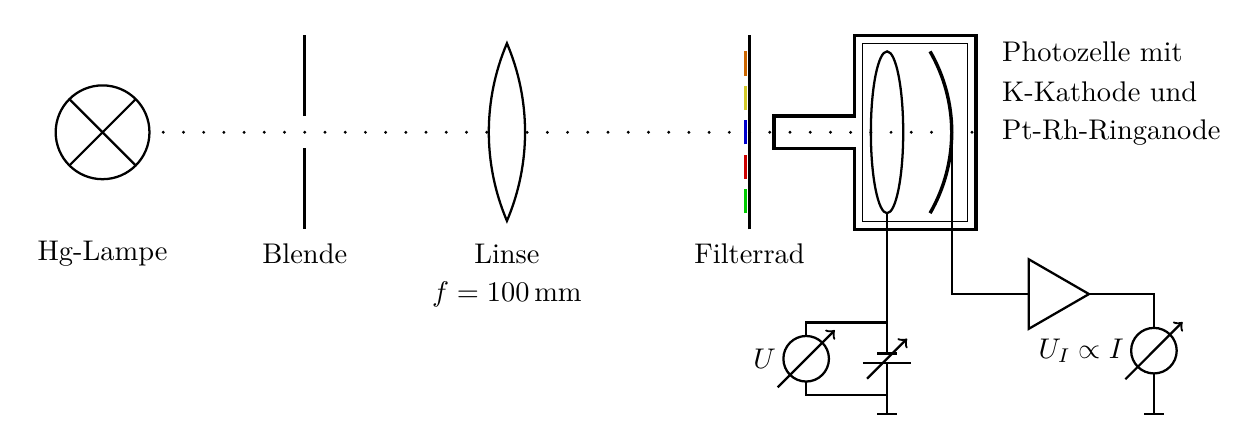
\includegraphics[width=0.8\linewidth]{photozelle_optikbank}
    \caption{Versuchsaufbau: Photoelektrische Bestimmung des planckschen Wirkungsquantum[\textbf{QUELLE!}]}
    \label{fig:photozelle_optikbank}
\end{figure}